\chapter{Óptica Geométrica}
\label{ch:geometrica}


La óptica geométrica fue la primera imagen conceptual que la humanidad elaboró para comprender la naturaleza de la luz. En esta concepción, la luz se entiende como compuesta de rayos que se propagan en línea recta a gran velocidad. 

En algún momento se llegó a pensar que dicha velocidad era infinita; sin embargo, a partir de las observaciones de los eclipses de Júpiter \cite{Romer1676} y de numerosos experimentos posteriores, sabemos, que la velocidad de la luz es finita.

Sin embargo, la propagación rectilínea de losrayos luminicos se ve modificada cuando la luz interactúa con los cuerpos materiales o, más precisamente, cuando atraviesa la frontera entre dos medios distintos. Como es manifiesto de la experiencia diaria en donde se observa como la luz se refleja en la superficies del agua, de los espejos, de los metales, \&c, y que también cambia de dirección al pasar de un medio a otro, como se observa en los objetos que se sumergidos en el agua y en los lentes. En general, cuando la luz experimenta un cambio de medio, se divide en una parte que retorna al medio de procedencia, y otra que se transmite al nuevo medio, dando lugar a los rayos transmitidos. Estos dos fenómenos se conocen como \textit{reflexión} y \textit{refracción} respectivamente.

La \emph{ley de la reflexión} fue conocida primero y mucho antes que la ley para la \emph{ley de la refracción}, siendo concebidas como leyes separadas y \textit{ad hoc}, en vez de responder a un principio natural. Definitivamente esta fue una gran incomodidad para los filosofos natirales que buscaban comprender la naturaleza de la luz, por la que la busqueda de un principio que explicara el comportamiento de la luz. 

Las investigaciones de Fermat dieron como resultado un principio natural por el cual se deducían las ya conocidas leyes de reflexión y refracción, así como la propagación rectilínea~\cite{bornwolf1999}.



\section{Principio de Fermat} 

\begin{center}
\textit{«Natura nihil agit frustra»}
\end{center}


La trayectoria $\Gamma$ que toma la luz para viajar de un punto $A$ a un punto $B$, de todas las posibles, es solo aquella que extrema el tiempo de trayecto



\begin{equation}
    \Gamma = \left\{ \Phi \mid \delta t(\Phi; A, B) = 0 \right\}        
    \label{eq:fermat_principle}
\end{equation}

donde $(\Phi, A, B)$ denota cualquier trayectoria $\Phi$ que une $A$ con $B$.

\begin{equation}
    n_0\ || AQ || + n' || QA' || = k,
    \label{eq:maxwell_condition_of_stigmatism_ovoid}
\end{equation}


\section{Ley Vectorial de Snell–Descartes} 


\begin{equation}
  \mathbf{k}_t = \frac{n_1}{n_2} \left\{ \mathbf{k}_i - (\mathbf{k}_i \cdot \mathbf{n})\mathbf{n} \right\} - \mathbf{n} \sqrt{ 1 - \left( \frac{n_1}{n_2} \right)^2 \left\{ 1 - (\mathbf{k}_i \cdot \mathbf{n})^2 \right\} }
  \label{eq:vectorial_law_of_snell_descartes}
\end{equation}



\section{Ovoides de Descartes} 

Las superficies cartesianas fueron introducidas por primera vez por el filósofo frances Rene Descartes en la \emph{DIOPTRIQUE} \cite{dioptrique}, como solución al problema del estigmátismo. 

Para que los rayos lúminosos que emerguen desde un punto $A$ convergan a otro punto $A'$, 
el tiempo que le toma a los rayos recorrer el trayecto de $A$ hasta $A'$ ha de ser el mismo, 
para que coincidad en lugar y tiempo. 
Cuando esta condición se cumple, al par $(A, A')$ se le conoce como \emph{par conjugado}. 

En general, la condición de que los rayos lúminosos converjan todos simultaneamente en un mismo punto, se le conoce como \emph{condición estigmática}~\cite{bornwolf1999}.

Considerando los rayos que emerguiendo de $A$ se refractan o se reflejan en cierta superficie $\Sigma$, y converguen todos al mismo punto $A'$, denotamos $\overline{AIA'}$ como el trayecto que realizan los rayos, siendo $I$ un punto de la superficie $\Sigma$.  Con $A$ y $A'$ fijos, solo los puntos de la superficie $\Sigma$ pueden ser seleccionados para cumplir la condición estigmatica. 

De tal manera, que exiguiendo matemáticamente la condicion estigmática para los rayos que siguen el trayecto anteriormente mencionado, se determina la familia de superficies $\Sigma$ que la satisfacen.  



Tales superficies son conocidas ampliamente en la literatura \emph{Ovoide de Descartes}, en atribución a el filosofo francés Rene Descartes, que escribio sobre ellas en la DIOPTRIQUE. 

La búsqueda matemática de esta superficie se hace exigiendo a la superficie que los rayos emitidos desde un punto $A$ lleguen todos al mismo tiempo a $A'$ independientemente del punto de la superficie que se tome como intermedio. Llamando al punto intermedio $I$ 



\begin{equation}
    n_0\ || AQ || + n' || QA' || = k,
    \label{eq:maxwell_condition_of_stigmatism}
\end{equation}


\begin{equation}
   f_\Sigma =  n_0\ || AQ || + n' || QA' || - k = 0,
\end{equation}


\begin{equation}
  f_{\Sigma}(x,y,z) = O G z^2 - 2(1 + S\varphi^2)z + (O + T\varphi^2)\varphi^2 = 0 
  \label{eq:implicit_ovoid_GOTS}
\end{equation}

\begin{equation}
  z(\varphi) = \frac{(O + T\varphi^2)\varphi^2}{1 + S\varphi^2 + \sqrt{1 + (2S - O^2G)\varphi^2}}
  \label{eq:parametrical_ovoid_z}
\end{equation}

\begin{equation}
  r(\varphi) = \sqrt{\varphi^2 - z^2(\varphi)} 
  \label{eq:parametrical_ovoid_r}
\end{equation}


La manera de referirse a un punto $Q$ de $\Sigma$ desde el punto $O$, se hace mediante el vector $\lvec{OQ}$, que junto con las ecuaciones paramétricas \ref{eq:parametrical_ovoid_z} y \ref{eq:parametrical_ovoid_r} se puede expresar en la forma: 


\begin{equation}
  \lvec{OQ} = z(\rho)\uvec{z} + r(\rho)\uvec{r}(\varphi),
  \label{eq:OQ_vector}
\end{equation}


Las leyes de la óptica geométrica permiten determinar, a partir de la dirección del rayo incidente y el punto de intersección del rayo con la superficie, la dirección del rayo transmitido o reflejado en dicho punto. Y no depende del punto en sí, sino de la normal de la superficie en ese punto, como es manifiesto de la ley vectorial~\eqref{eq:vectorial_law_of_snell_descartes} deducida desde el \emph{principio de Fermat}~\cite{bornwolf1999}.

Así, procedemos a escribir el vector normal de incidencia para un punto cualesquiera $Q \in \Sigma$ parametrizado por $(\rho, \phi)$. 

Sea $P$ el origen de el rayo incidente y $Q(\rho, \phi)$ el punto de intersección del rayo con la superficie $\Sigma$, es manifiesto que el vector unitario de incidencia $\uvec{u}$ es el vector unitario de $\lvec{AQ}$, es decir 



\begin{equation}
  \uvec{u} = \frac{\lvec{PQ}}{\lVert \lvec{PQ} \rVert}.
  \label{eq:def_of_u}
\end{equation}

Sean $(z_0, r_0, \varphi_0)$ las coordenadas de $P$, de modo que 

\begin{equation}
  \lvec{OP} = z_0\uvec{z} + r_0 \uvec{r}(\varphi_0)
  \label{eq:def_OP_where_P_is_any_point_of_space}
\end{equation}


Contruimos pues el vector $\lvec{OQ}$, 

\begin{equation}
  \lvec{PQ} = \lvec{OQ} - \lvec{OP}
\end{equation}

\begin{equation}
 \lvec{PQ} = (z(\rho) - z_0)\,\uvec{z}
+ \bigl(r(\rho) - r_0 \cos\Delta\varphi\bigr)\,\uvec{r}(\varphi)
+ r_0 \sin\Delta\varphi\,\uvec{\varphi}(\varphi), 
  \label{eq:explicit_PQ}
\end{equation}

donde $\Delta \varphi$ es la diferencia $\varphi - \varphi_0$. 


Calculamos la norma de $\lvec{PQ}$


\begin{equation}
  \lVert \lvec{PQ} \rVert^2
= \rho^2 - 2 z(\rho) z_0 + z_0^2
+ r_0^2 - 2 r(\rho) r_0 \cos\Delta\varphi,
\end{equation}

y finalmente obtenemos el vector normal de incidencia


% Vecotres u y u'.

\begin{equation}
   \uvec{u}
  =
  \frac{
  (z(\rho) - z_0)\,\uvec{z}
  + \bigl(r(\rho) - r_0 \cos\Delta\varphi\bigr)\,\uvec{r}(\varphi)
  + \bigl(r_0 \sin\Delta\varphi\bigr)\,\uvec{\varphi}(\varphi)
  }{
  \sqrt{(z(\rho) - z_0)^2 + r(\rho)^2 + r_0^2 - 2 r(\rho) r_0 \cos\Delta\varphi}
  }.
  \label{eq:u_for_any_P}
\end{equation}


\begin{equation}
   \uvec{u}'
  =
  \frac{
  (z(\rho) - z_i)\,\uvec{z}
  + \bigl(r(\rho) - r_i \cos\Delta\varphi\bigr)\,\uvec{r}(\varphi)
  + \bigl(r_i \sin\Delta\varphi\bigr)\,\uvec{\varphi}(\varphi)
  }{
  \sqrt{(z(\rho) - z_i)^2 + r(\rho)^2 + r_i^2 - 2 r(\rho) r_i \cos\Delta\varphi}
  }.
  \label{eq:u_prime_for_any_P}
\end{equation}


Si los puntos $P$ y $P'$ viven en el eje óptico, la expresión para $\uvec{u}$ se simplifica como: 

\begin{equation}
  \uvec{u} = \frac{(z(\rho) - z_i)\uvec{z} + r(\rho)\uvec{r}(\varphi)}{\sqrt{\rho^2 - 2z(\rho)z_i + z_i^2}}  
  \label{eq:u_for_P_in_optical_axis}
\end{equation}



\begin{equation}
  \uvec{u}' = \frac{(z(\rho) - z_0)\uvec{z} + r(\rho)\uvec{r}(\varphi)}{\sqrt{\rho^2 - 2z(\rho)z_0 + z_0^2}}  
  \label{eq:u_prime_for_P_in_optical_axis}
\end{equation}


Cuando $P$ esta en el plano $(z, r)$, se cumple que $\Delta \varphi = 0$, de tal manera que $\uvec{u}$ toma la forma 





Procedemos ahora con el cálculo de la normal, en un punto $Q$ parametrizado por  $(\rho, \phi)$, denotemos al vector normal en el punto $Q=Q(\rho, \varphi)$ como $\uvec{n}$, y construyamos un vector $\vec{N}$ proporcional a $\uvec{n}$ 




\[ 
  \vec{N} = \frac{\partial \vb{r}_\Sigma}{\partial \rho} \times \frac{\partial \vb{r}_\Sigma}{\partial \phi}
\]


\[
\vec{N}(\rho,\varphi)
=\frac{\partial \lvec{OQ}}{\partial \rho}\times \frac{\partial \lvec{OQ}}{\partial \varphi}
= r(\rho)\,r'(\rho)\,\uvec{z}-r(\rho)\,z'(\rho)\,\uvec{r}(\varphi)
= r(\rho)\Bigl(r'(\rho)\,\uvec{z}-z'(\rho)\,\uvec{r}(\varphi)\Bigr),
\]

donde hemos usado el hecho de que


\[
\frac{\partial \lvec{OQ}}{\partial \rho}
= z'(\rho)\,\uvec{z}+r'(\rho)\,\uvec{r}(\varphi),
\qquad
\frac{\partial \lvec{OQ}}{\partial \varphi}
= r(\rho)\,\uvec{\varphi}(\varphi).
\]

La norma de $\vec{N}$ esta dada por

\[
|\lvec{N}|
= r(\rho)\sqrt{(r'(\rho))^2+(z'(\rho))^2}
\]



De esta manera, obtenemos el vector unitario $\uvec{N}$, desde la definición:

\[
\uvec{n}(\rho,\varphi)=\frac{\lvec{N}}{|\lvec{N}|},
\]

por lo tanto,

\begin{equation}
\uvec{N}(\rho,\varphi) = \frac{r'(\rho)\,\uvec{z}-z'(\rho)\,\uvec{r}(\varphi)}{\sqrt{(r'(\rho))^2+(z'(\rho))^2}}.
  \label{eq:N_ovoid_rho_and_phi}
\end{equation}


\begin{equation}
    \uvec N(Q) = \frac{\bm \nabla f_\Sigma(Q)}{|| f_\Sigma(Q)||}
\end{equation}


Con esto quedan establecidas las cantidades geométricas esenciales para estudiar
la formación de imágenes en superficies cartesianas estigmáticas: la
parametrización de la superficie, los vectores direccionales de incidencia y
refracción, y la normal local. Estas expresiones constituyen además la base
operativa para el problema vectorial desarrollado en los capítulos siguientes,
en particular para la definición de la base local de Fresnel y el cálculo de la
transformación de polarización en la interfaz.

\subsection{Comparación de foco de una superficie cartesiana y una superficie esférica equivalente}

Para contrastar la capacidad de formación puntual de imagen, se comparó por
trazado de rayos 3D una superficie cartesiana estigmática con una superficie
esférica equivalente, ambas referidas al mismo par conjugado axial
$A\rightarrow A'$. La superficie cartesiana está construida para mantener la
igualdad de camino óptico entre $A$ y $A'$, por lo que su comportamiento es
estigmático para ese par objeto--imagen; en cambio, la superficie esférica solo
reproduce el enfoque paraxial axial y, fuera de ese límite, introduce
aberración geométrica. Esta diferencia se observa directamente en el corte
meridional $r$--$z$ y en los spot diagrams del plano detector.

\begin{figure}[htbp]
\centering
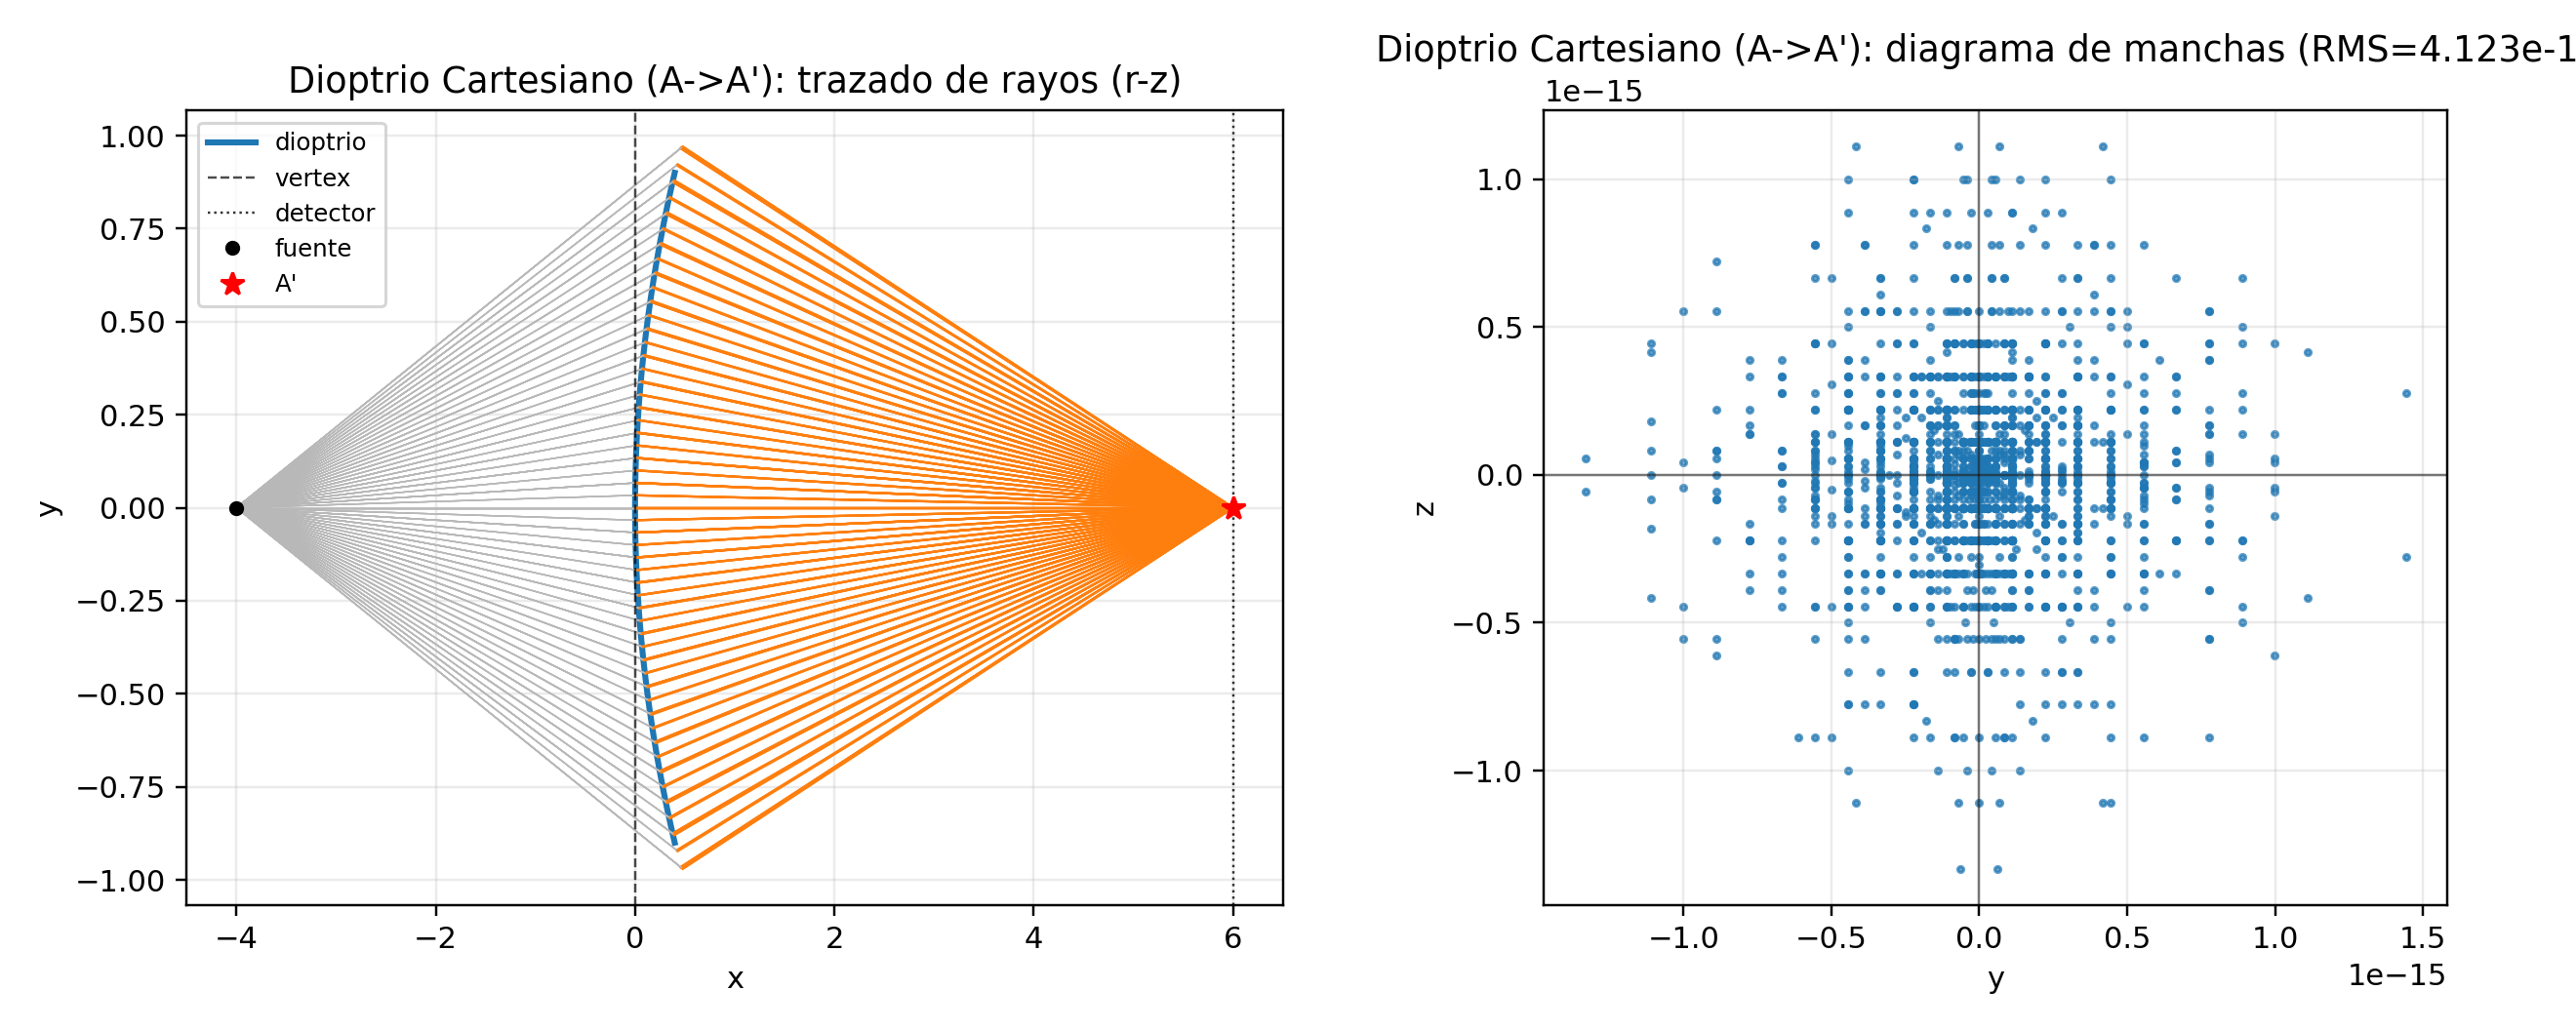
\includegraphics[width=0.90\textwidth]{figures/results_of_simulation/raytrace/case_focus_cartesian_unified.png}
\caption{Dioptrio cartesiano, fuente en $A$ y detector en $A'$: en el corte $r$--$z$ se observa convergencia al plano focal y un spot prácticamente puntual (RMS numéricamente cercano a cero).}
\label{fig:raytrace_focus_cartesian}
\end{figure}

\begin{figure}[htbp]
\centering
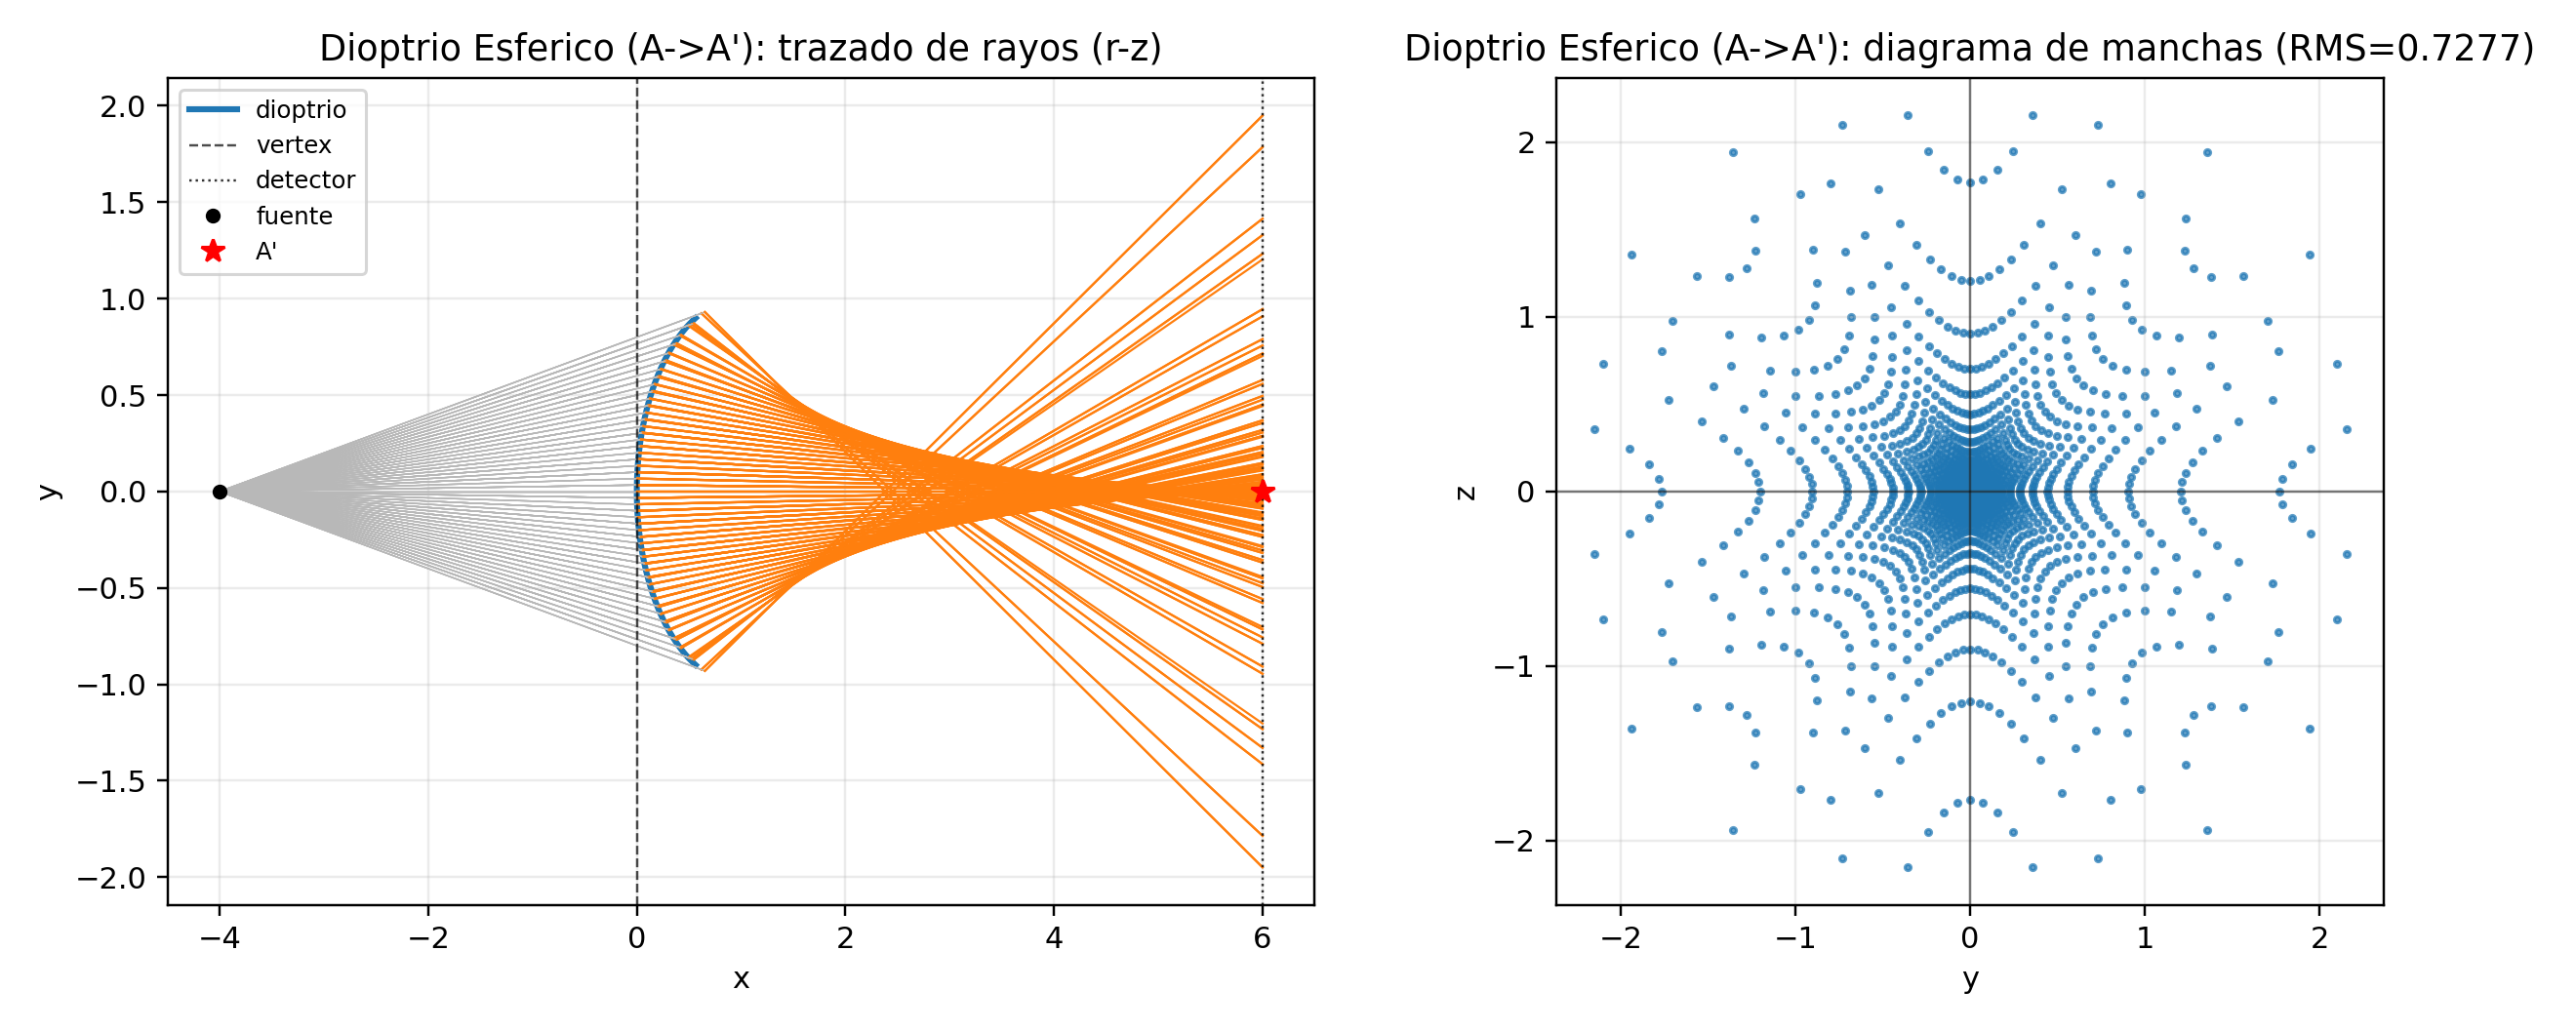
\includegraphics[width=0.90\textwidth]{figures/results_of_simulation/raytrace/case_focus_spherical_unified.png}
\caption{Dioptrio esférico para el mismo par $A\rightarrow A'$: comparte el foco paraxial axial, pero el spot muestra apertura transversal por aberración esférica.}
\label{fig:raytrace_focus_spherical}
\end{figure}

\begin{figure}[htbp]
\centering
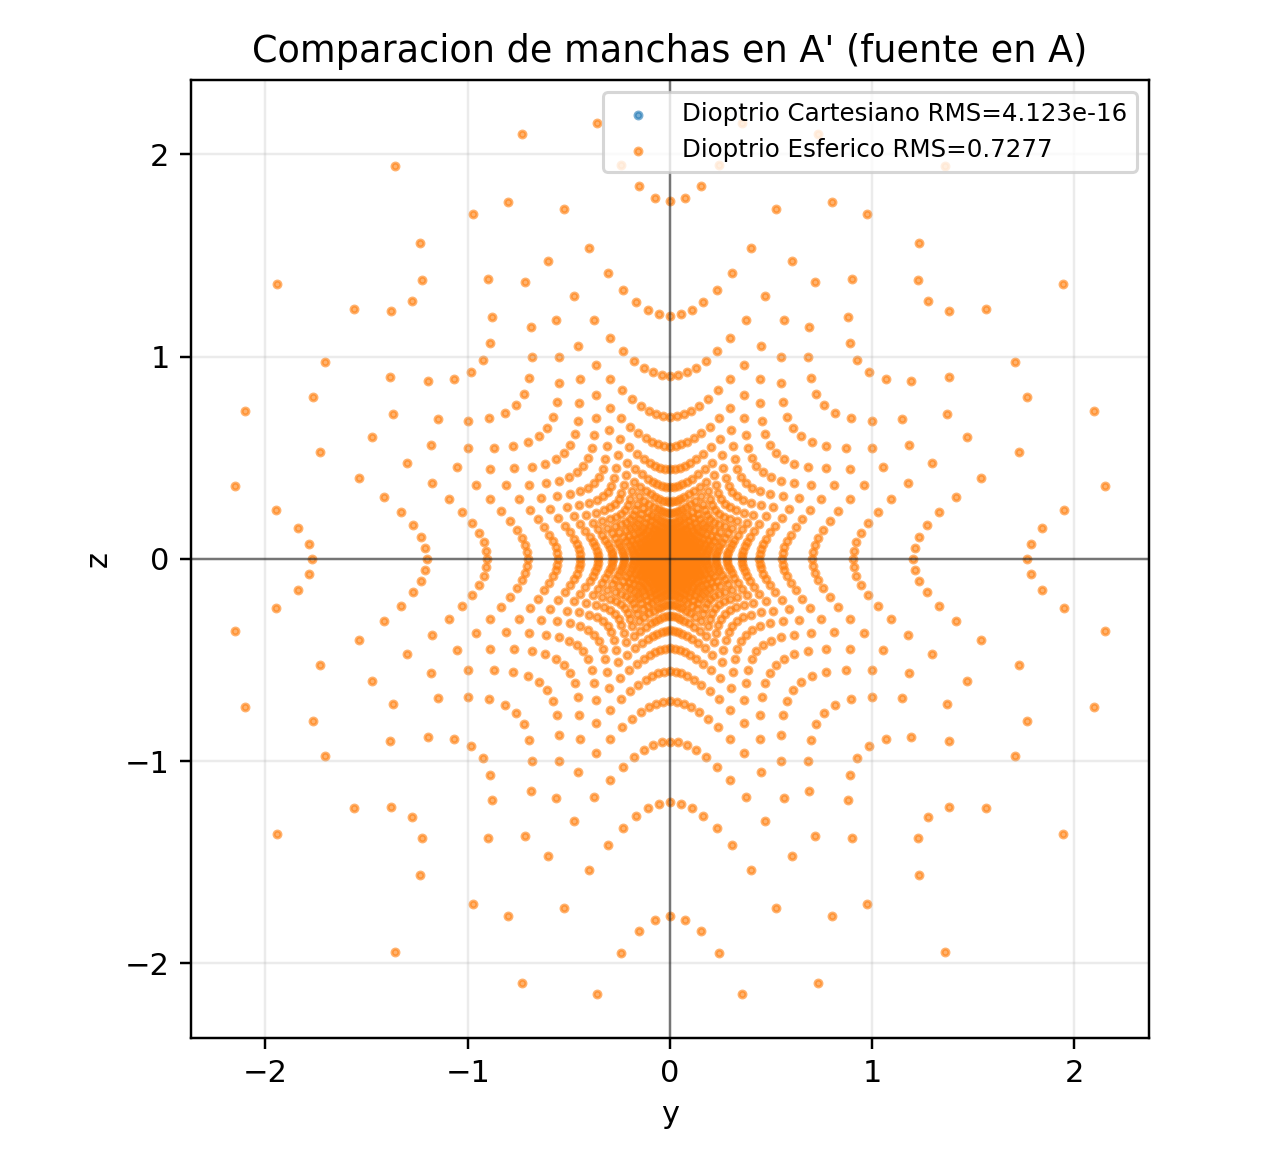
\includegraphics[width=0.72\textwidth]{figures/results_of_simulation/raytrace/case_focus_spot_compare.png}
\caption{Comparación directa de spot diagrams en $A'$ para fuente en $A$: el dioptrio cartesiano concentra los rayos, mientras que el esférico produce una mancha extendida.}
\label{fig:raytrace_focus_spot_compare}
\end{figure}

\begin{figure}[htbp]
\centering
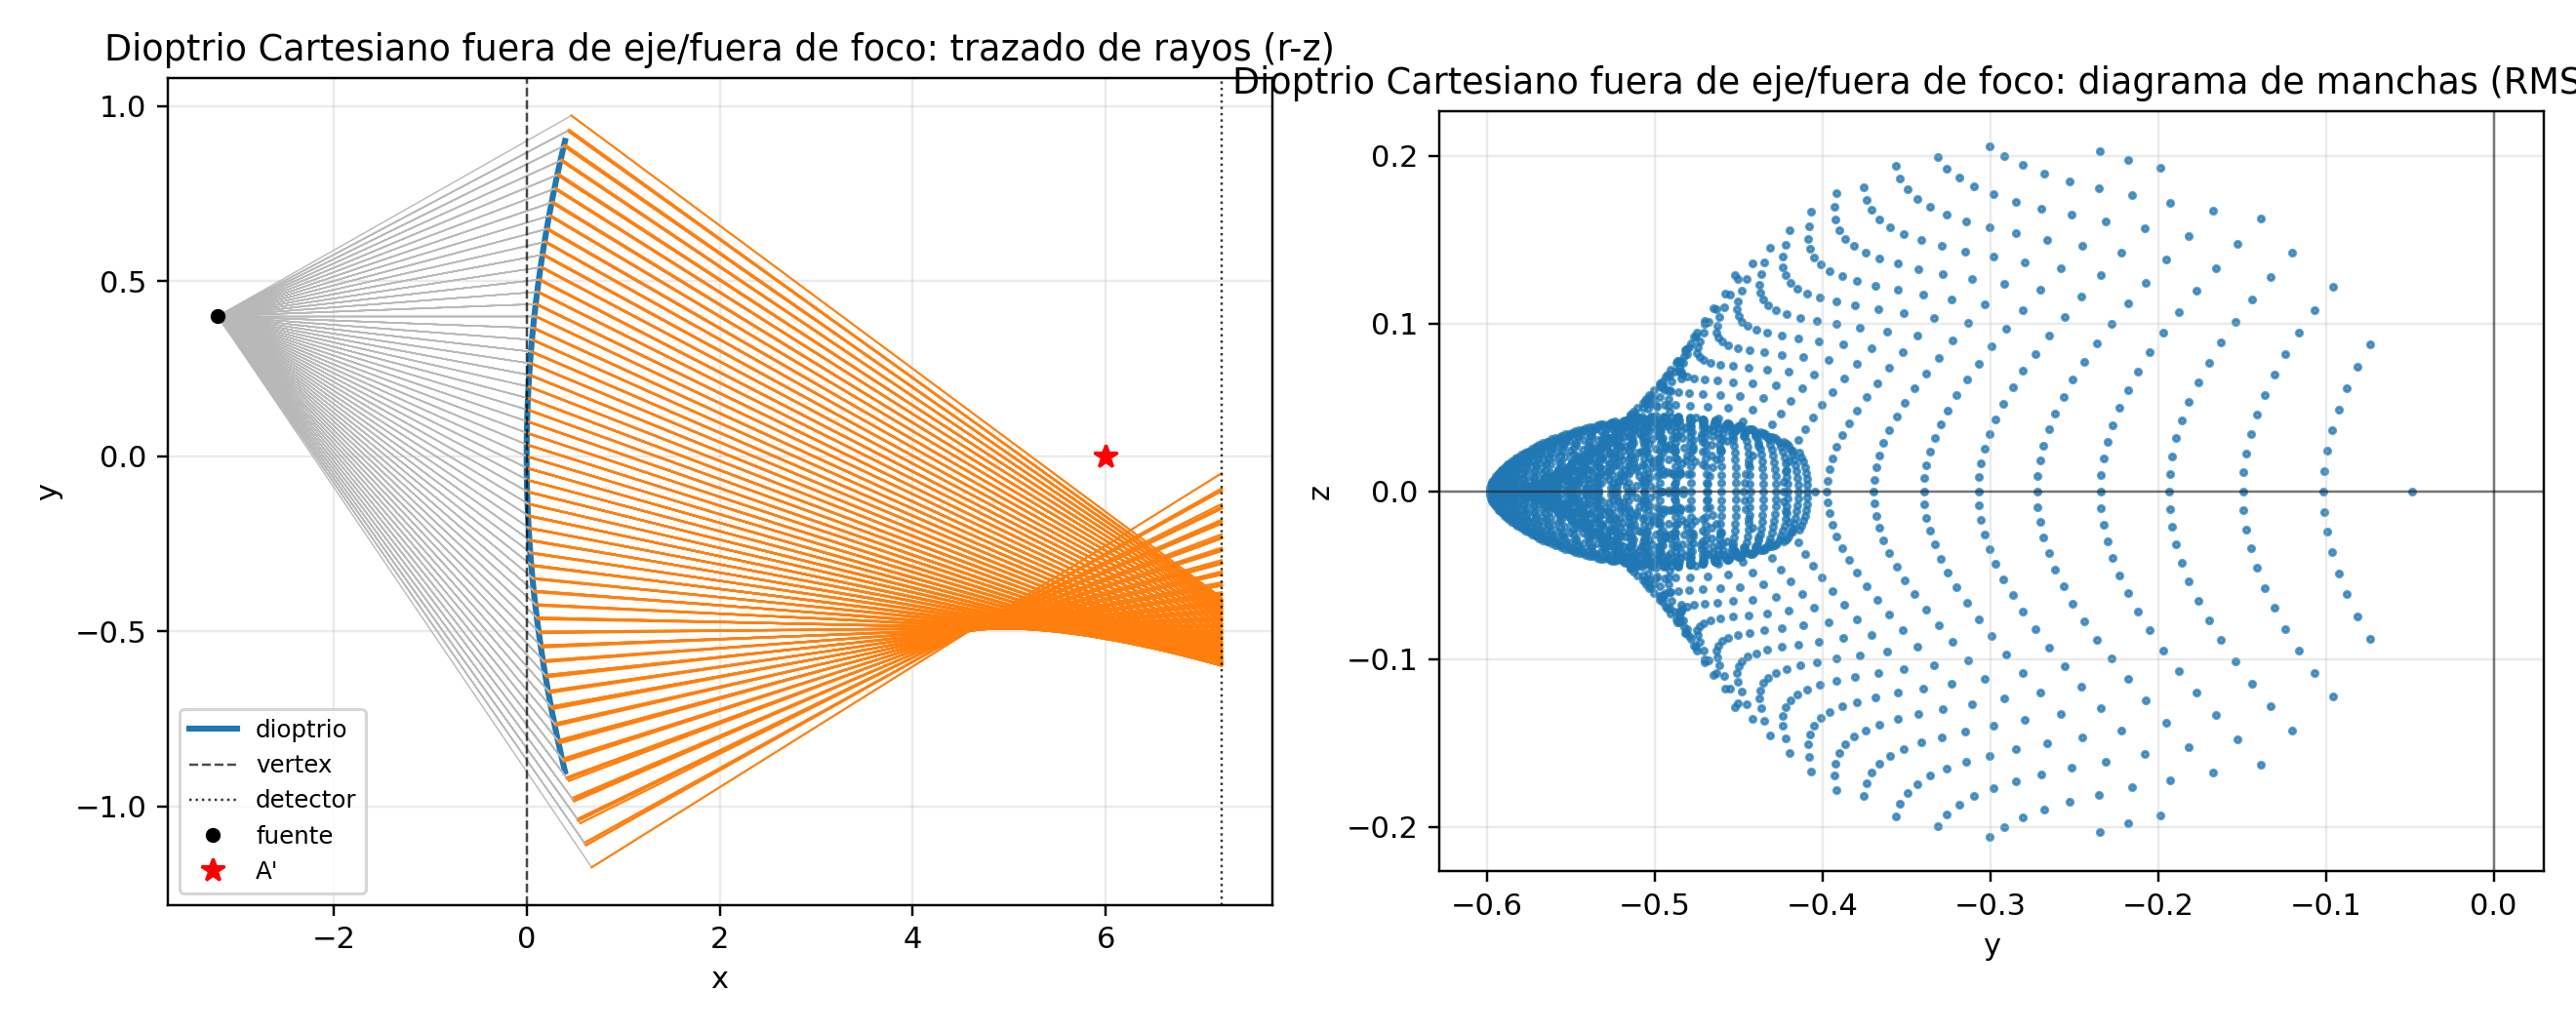
\includegraphics[width=0.90\textwidth]{figures/results_of_simulation/raytrace/case_offaxis_offfocus_unified.png}
\caption{Dioptrio cartesiano en condición fuera de eje y fuera de foco: el trazado en $r$--$z$ y el spot diagram muestran pérdida de concentración al romperse la condición conjugada nominal.}
\label{fig:raytrace_offaxis_offfocus}
\end{figure}

% =========ÓPTICA ONDULATORIA =============
